
% Preamble
\documentclass[12pt]{report}

% Packages
\usepackage[english]{babel}
% unicdoe is the default since 2018
\usepackage{simple_report}

\usepackage{calligra} % used for authors
\usepackage{miama}
% dummy data
% https://texblog.org/2011/02/26/generating-dummy-textblindtext-with-latex-for-testing/
\usepackage{blindtext}
\usepackage{lipsum}

% Document
\begin{document}
    \begin{simplefrontpage}{Programming}{MediumBlue}{white}
        \begin{simpletitle}{This is a title}{This is a description}{images/moon_deer1.png}
            {\large\bfseries Double O Seven} \hspace{10mm}
			\calligra{\LARGE Caption Sparrow}\\ \medskip \medskip
			\fmmfamily{\huge Legolas the Elf}
        \end{simpletitle}
    \end{simplefrontpage}

    \simplechapter{New Tool}
    This is a simple tool.

    \section{Acronyms}
	\blindtext

	\begin{figure}[htb]
		\centering
		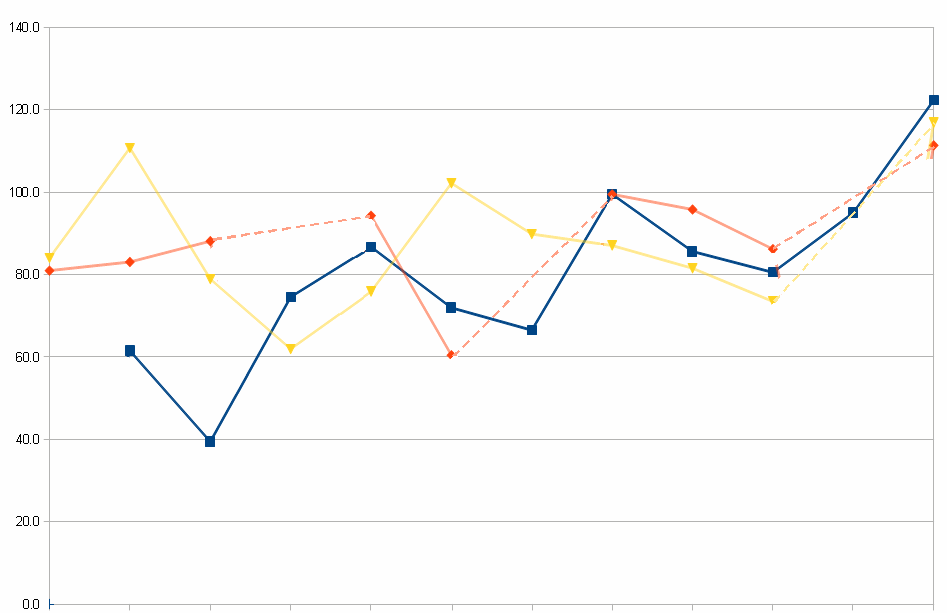
\includegraphics[width=1\textwidth]{images/figure1}
		\centering
		\textcolor{ctbPurpleDark}{\textbf{\caption{Figure Description}\label{fig:chart1}}}
		% caption and label have to stay togeter, otherwise the label is not there.
	\end{figure}

    The chart~\ref{fig:chart1} is nice, imported.

	\section{Excel}
	\blindtext[2] % repeat 2 times

    \begin{figure}[htb]
		\centering
		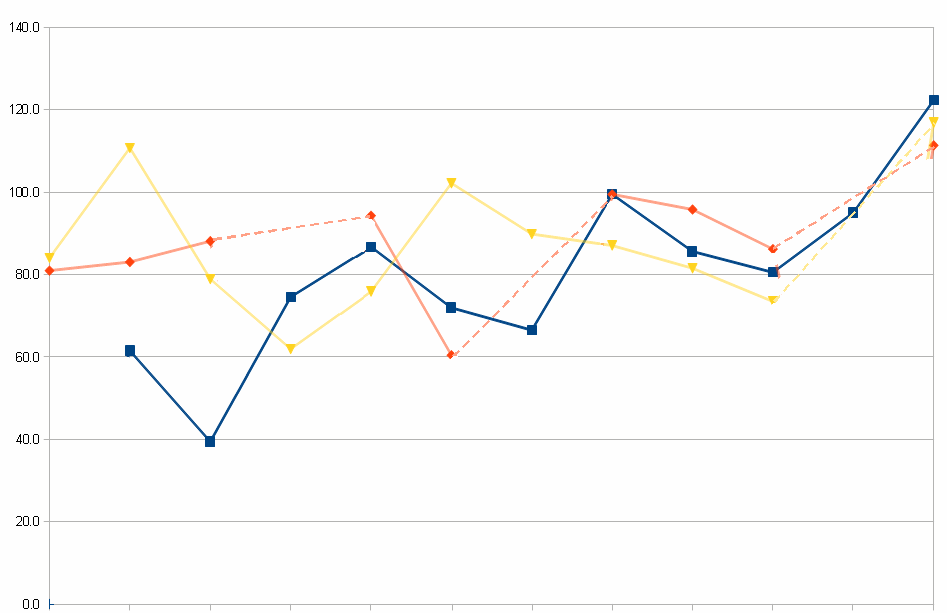
\includegraphics[width=1\textwidth]{images/figure1}
		\centering
		\textcolor{ctbPurpleDark}{\textbf{\caption{Figure Description}\label{fig:2}}}
	\end{figure}
	The chart~\ref{fig:2} is nice, imported.

	\lipsum

    \simplechapter{Next New Tool}
    This is check header
    \section{Python}
	\lipsum[1-2] % paragraphs

    \section{Scala}
	\blindtext[5]

% testing code for title
%    \setlength{\TPHorizModule}{1mm}
%     \setlength{\TPVertModule}{1mm}
%\begin{simpletitle}{This is a title}{This is a description}{images/panda.jpg}
%            { \large\bfseries Firstname Lastname}
%        \end{simpletitle}
\end{document}
